%!TEX root=../../autopilot.tex
\section{Network Bandwidth}
\label{sec:bandwidth}


\begin{margintable}[-6.6cm]
\caption{Terminal Specs}
\label{tab:terminal}
\noindent\begin{tabularx}{\linewidth}{rR}
\toprule
    CPU & AMD FX-4300 \\
    CPU Speed & 3.8GHz \\
    Memory & 8GB \\
    Ethernet & 1Gbit/s \\
    Switch & NETGEAR GSS116E \\
\bottomrule
\end{tabularx}
\end{margintable}

\begin{marginfigure}[-0.4cm]
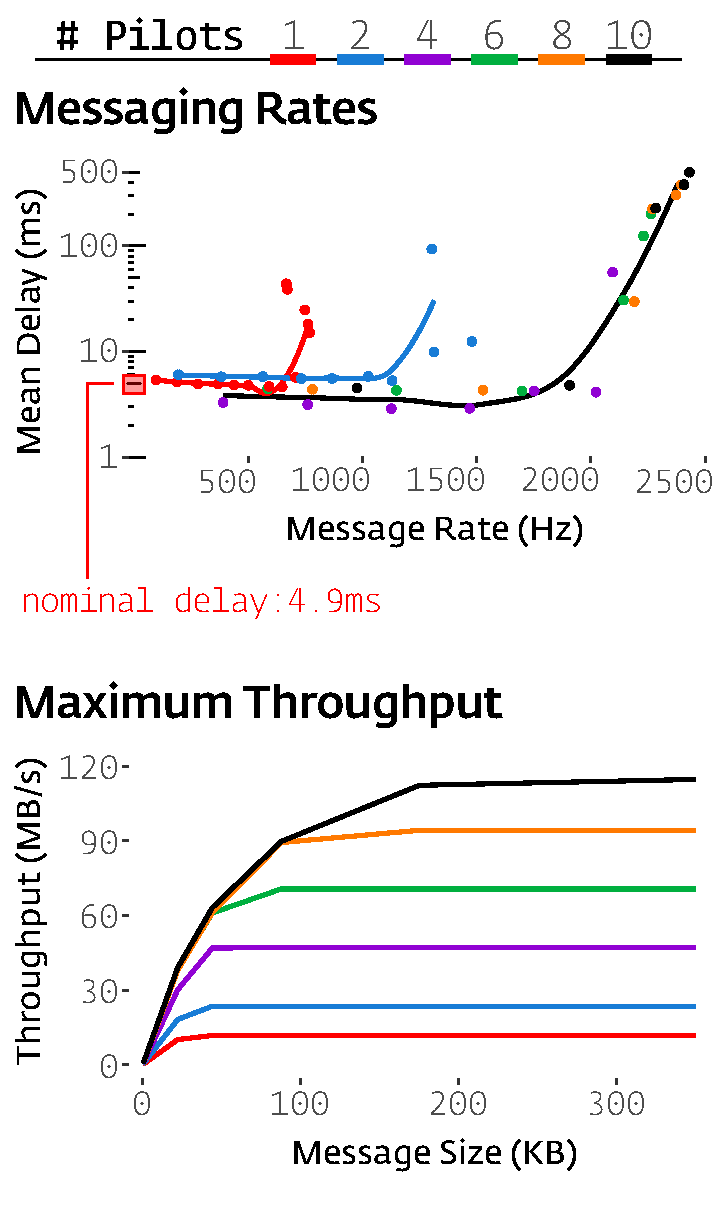
\includegraphics[]{figures/test_net_combined.pdf}

\caption{Network latency (top) and throughput (bottom) tests. Each point in the latency test represents the mean rate and delay of 5,000 255 Byte messages. Throughput (bottom) was calculated as the product of message rate and message size, and is displayed for a test that requested different numbers of pilots (colors) to send messages of different size to the terminal.}
\label{fig:speed}
\end{marginfigure}

To demonstrate yet another modality of use, we tested network capacity using Autopilot's \href{http://docs.auto-pi-lot.com/autopilot.core.gui.html#autopilot.core.gui.Bandwidth_Test}{\texttt{Bandwidth\_Test}} widget, an action available from the Terminal GUI's \texttt{tests} menu. This test requests that a set of selected pilots send messages at a range of selected frequencies and payload sizes back to the terminal. The messages pass through four networking objects en route: the stations and network nodes running the test for both the terminal and pilots (See Figure \ref{fig:datastreams}). Delay is measured as the duration between the creation of the message at the sender and the processing of the message at the receiver. The Pis and terminal were synchronized on common NTP servers to align timestamps. 

First we tested the limits of our terminal's ability to receive messages from the 10 pilots that it controls. Our terminal is a modest desktop (complete with a vintage 2012 CPU, see Table \ref{tab:terminal}) with ethernet connections to 10 Raspberry Pi 3b's through a network switch. We first tested the rate at which the Pi 3b's and our terminal could send and process typical (\texttt{255 Byte}) messages without a data payload (Figure \ref{fig:speed}, top). A single Pi was capable of sending at a maximum rate of \texttt{707 Hz} without exceeding its nominal mean delay of \texttt{4.9} ($\pm$ \texttt{0.47}) ms. Adding additional Pis did not cause increased delay until the total sending rate surpassed roughly \texttt{2000 Hz}. These are the rate limits of sending and receiving messages, respectively.

As we increased the size of each individual message by including payloads of generated data (Figure \ref{fig:speed}, bottom), the rate of messaging decreased, but the total throughput (\texttt{message rate (Hz) * size (Bytes)}) saturated linearly as a multiple of the number of sending Pis. The Raspberry Pi 3b has a shared USB/Ethernet Bus, and thus appears to have a relatively limited \texttt{11.8MB/s} throughput.

\begin{marginfigure}[0.1cm]
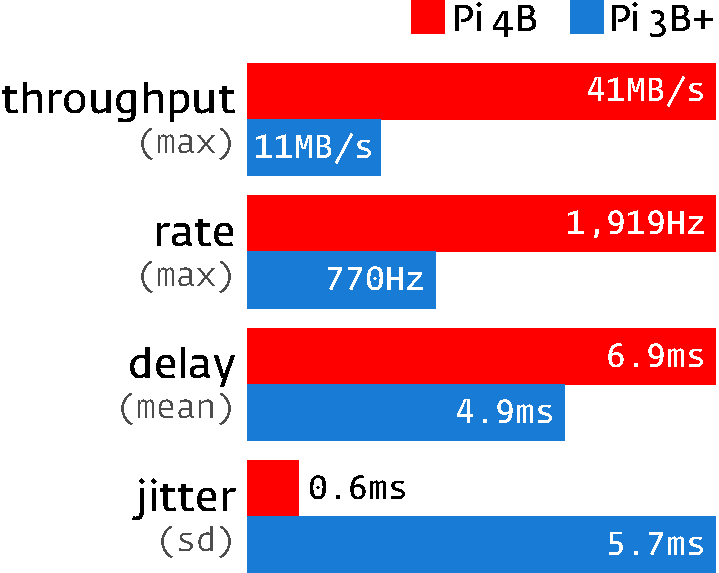
\includegraphics[]{figures/test_4_comparison.pdf}
\caption{The Raspberry Pi 4's gigabit ethernet bus markedly improves network performance.}
\label{fig:netcomparison}
\end{marginfigure}

Fortunately, the Raspberry Pi 4 has an independent \href{https://www.raspberrypi.org/magpi/raspberry-pi-4-specs-benchmarks/}{gigabit ethernet bus}. On a Raspberry Pi 4, Autopilot has a \texttt{41MB/s} maximum throughput and a \texttt{1,919Hz} maximum messaging rate (Figure \ref{fig:netcomparison}). We observed a slightly higher messaging delay with the Raspberry Pi 4 (\texttt{6.9ms} vs. \texttt{4.9ms} Raspberry Pi 3B+). We note that the NTP synchronization method we used to measure delays has a margin of error on the order of milliseconds. 

Autopilot's networking modules are capable of supporting the infrastructure of next-generation behavioral neuroscience experiments. Our humble terminal was capable of receiving the full \texttt{114.6MB/s} of 10 Pis without sign of saturation, and a Raspberry Pi 4 is capable of sending data at \texttt{41MB/s}. This bandwidth makes Autopilot capable of streaming raw Calcium imaging\sidenote{2-Photon:  5.9MB/s\\ \noindent (12 bits * 512x512 resolution * 15Hz)} and electrophysiological data from modern high-density probes\sidenote{Neuropixels: 14.4MB/s\citep{junFullyIntegratedSilicon2017}\\\noindent(10 bits * 30kHz * 384 channels)}. The delay between sending and processing messages over 4 hops in a network (\texttt{4.9ms}) is less than the latency with which comparable systems (Figure \ref{fig:lags}) process triggers when connected directly via serial.

Finally, while Autopilot typically operates in a "TCP-like" protocol---resending messages until they have been confirmed as received---these tests were run with an optional "UDP-like" protocol which does not check for confirmation. Across the approximately 2.5 million messages sent during these tests only \texttt{537} were dropped (and only during tests which saturated rate or bandwidth capacity), giving Autopilot a delivery rate of \texttt{99.98\%} in "UDP" mode. By design, delivery rate is guaranteed to be 100\% in "TCP" mode.